\documentclass{article}
\usepackage{pgfplots}
\usepackage{subcaption}
\usepackage{graphicx}
\usepackage{geometry}
\usepackage{float}
\usepackage{xcolor}
\usepackage{amsmath}
\usepackage{caption}

% 设置页面边距
\geometry{a4paper, margin=1in}

% 设置pgfplots样式
\pgfplotsset{
    compat=1.17,
    width=12cm,
    height=8cm,
    grid style={dashed, gray!30},
    every axis/.append style={
        thick,
        font=\small
    },
    every axis title/.append style={font=\bfseries\large},
    every axis label/.append style={font=\bfseries},
    legend style={
        at={(0.98,0.98)},
        anchor=north east,
        font=\small
    }
}

% 定义颜色
\definecolor{cfoBlue}{HTML}{2E86AB}
\definecolor{krumOrange}{HTML}{F18F01}
\definecolor{trimmedRed}{HTML}{C73E1D}
\definecolor{medianGreen}{HTML}{6A994E}
\definecolor{trustPurple}{HTML}{A23B72}
\definecolor{bulyanBrown}{HTML}{BC4B51}

\begin{document}

\title{Multi-Agent Byzantine Fault Tolerant Consensus System \\ Comparison Visualization}
\author{}
\date{}
\maketitle

\begin{abstract}
This document presents LaTeX-generated comparison figures for multi-agent Byzantine fault tolerant consensus systems, including comparisons with traditional BFT algorithms, federated learning methods, multi-agent consensus approaches, and tolerance-accuracy trends.
\end{abstract}

\section{Comparison with Traditional BFT Consensus Algorithms}

\begin{figure}[H]
\centering
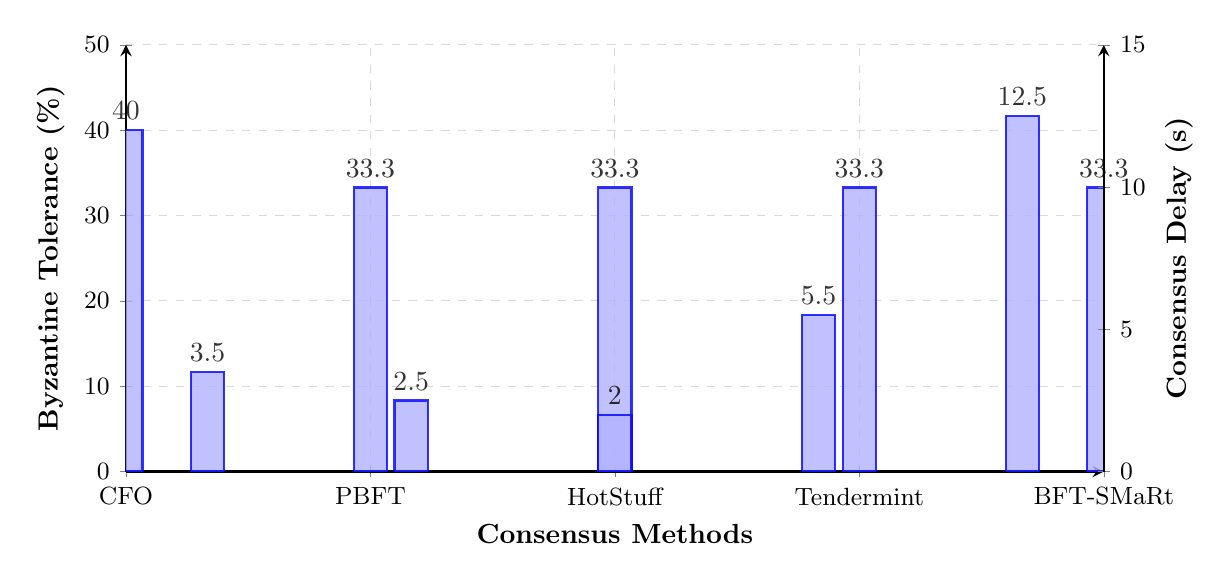
\begin{tikzpicture}
\begin{axis}[
    width=14cm,
    height=7cm,
    ybar=5pt,
    bar width=12pt,
    symbolic x coords={CFO,PBFT,HotStuff,Tendermint,BFT-SMaRt},
    xtick=data,
    ylabel={Byzantine Tolerance (\%)},
    xlabel={Consensus Methods},
    ymin=0, ymax=50,
    grid=both,
    grid style={dashed, gray!30},
    axis lines=left,
    axis line style={thick},
    every axis plot/.append style={fill=cfoBlue, opacity=0.8},
    nodes near coords,
    nodes near coords align={above},
    every node near coord/.append style={font=\bfseries, color=black}
]

\addplot coordinates {
    (CFO,40)
    (PBFT,33.3)
    (HotStuff,33.3)
    (Tendermint,33.3)
    (BFT-SMaRt,33.3)
};

\end{axis}

\begin{axis}[
    width=14cm,
    height=7cm,
    ybar=5pt,
    bar width=12pt,
    symbolic x coords={CFO,PBFT,HotStuff,Tendermint,BFT-SMaRt},
    xtick=data,
    ylabel={Consensus Delay (s)},
    ymin=0, ymax=15,
    axis y line=right,
    axis x line=none,
    every axis plot/.append style={fill=trustPurple, opacity=0.8},
    nodes near coords,
    nodes near coords align={above},
    every node near coord/.append style={font=\bfseries, color=black}
]

\addplot coordinates {
    (CFO,3.5)
    (PBFT,2.5)
    (HotStuff,2)
    (Tendermint,5.5)
    (BFT-SMaRt,12.5)
};

\end{axis}
\end{tikzpicture}
\caption{Comparison with Traditional BFT Consensus Algorithms. CFO achieves 40\% Byzantine tolerance with 3.5s consensus delay (algorithm only, excluding 60-90s for 30 sequential LLM API calls).}
\label{fig:bft_comparison}
\end{figure}

\section{Comparison with Federated Learning Byzantine Defense Methods}

\begin{figure}[H]
\centering
\begin{subfigure}{0.48\textwidth}
\centering
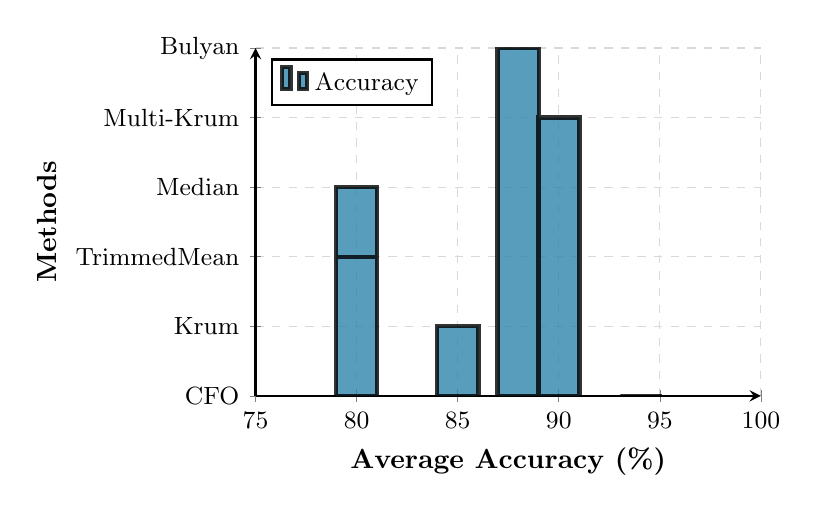
\begin{tikzpicture}
\begin{axis}[
    width=8cm,
    height=6cm,
    ybar,
    bar width=15pt,
    symbolic y coords={CFO,Krum,Trimmed\\Mean,Median,Multi-Krum,Bulyan},
    ytick=data,
    xlabel={Average Accuracy (\%)},
    ylabel={Methods},
    xmin=75, xmax=100,
    grid=both,
    grid style={dashed, gray!30},
    axis lines=left,
    axis line style={thick},
    legend pos=north west
]

\addplot[fill=cfoBlue, opacity=0.8, draw=black, line width=1.5pt] coordinates {
    (94.08,CFO)
    (85,Krum)
    (80,Trimmed\\Mean)
    (80,Median)
    (90,Multi-Krum)
    (88,Bulyan)
};

\legend{Accuracy}

\end{axis}
\end{tikzpicture}
\caption{Prediction Accuracy Comparison}
\label{fig:federated_accuracy}
\end{subfigure}
\hfill
\begin{subfigure}{0.48\textwidth}
\centering
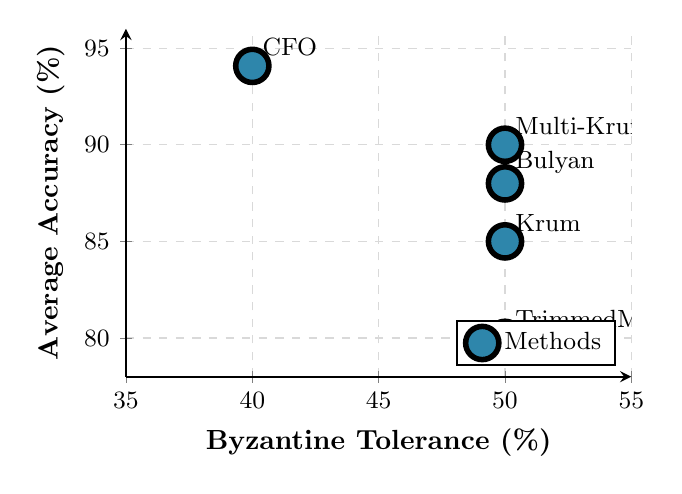
\begin{tikzpicture}
\begin{axis}[
    width=8cm,
    height=6cm,
    xlabel={Byzantine Tolerance (\%)},
    ylabel={Average Accuracy (\%)},
    xmin=35, xmax=55,
    ymin=78, ymax=96,
    grid=both,
    grid style={dashed, gray!30},
    axis lines=left,
    axis line style={thick},
    legend pos=south east
]

\addplot[
    only marks,
    mark=*,
    mark size=6pt,
    color=cfoBlue,
    draw=black,
    line width=2pt
] coordinates {
    (40,94.08)
    (50,85)
    (50,80)
    (50,80)
    (50,90)
    (50,88)
};

\addlegendentry{Methods}

% 添加标签
\node at (axis cs:40,94.08) [above right] {CFO};
\node at (axis cs:50,85) [above right] {Krum};
\node at (axis cs:50,80) [above right] {Trimmed\\Mean};
\node at (axis cs:50,80) [below right] {Median};
\node at (axis cs:50,90) [above right] {Multi-Krum};
\node at (axis cs:50,88) [above right] {Bulyan};

\end{axis}
\end{tikzpicture}
\caption{Tolerance vs Accuracy}
\label{fig:federated_scatter}
\end{subfigure}
\caption{Comparison with Federated Learning Byzantine Defense Methods}
\label{fig:federated_comparison}
\end{figure}

\section{Comparison with Multi-Agent Consensus Methods}

\begin{figure}[H]
\centering
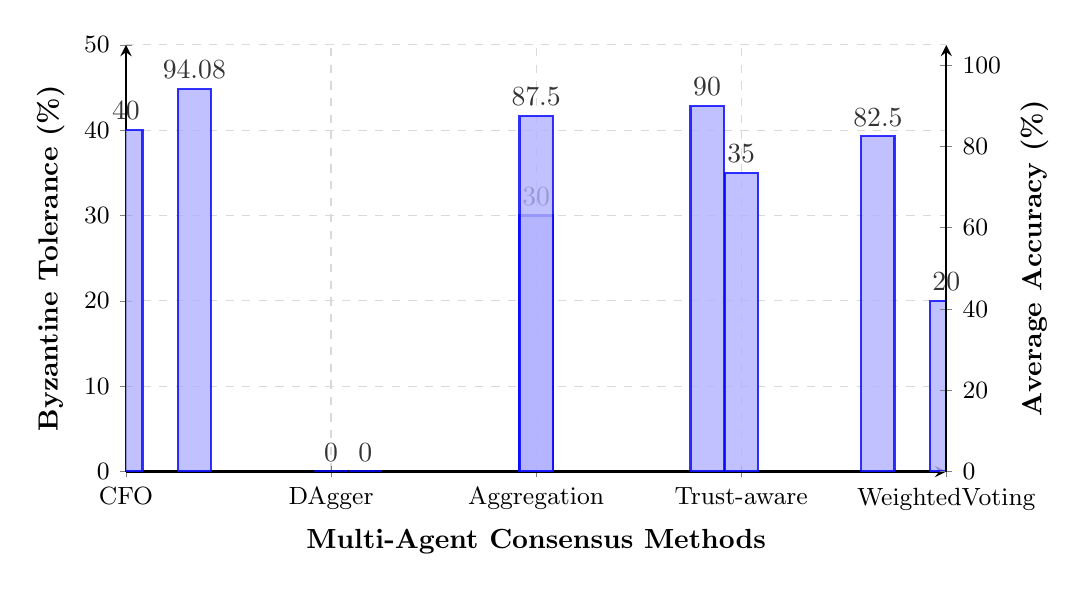
\begin{tikzpicture}
\begin{axis}[
    width=12cm,
    height=7cm,
    ybar=5pt,
    bar width=12pt,
    symbolic x coords={CFO,DAgger,Aggregation,Trust-aware,Weighted\\Voting},
    xtick=data,
    ylabel={Byzantine Tolerance (\%)},
    xlabel={Multi-Agent Consensus Methods},
    ymin=0, ymax=50,
    grid=both,
    grid style={dashed, gray!30},
    axis lines=left,
    axis line style={thick},
    every axis plot/.append style={fill=cfoBlue, opacity=0.8},
    nodes near coords,
    nodes near coords align={above},
    every node near coord/.append style={font=\bfseries, color=black}
]

\addplot coordinates {
    (CFO,40)
    (DAgger,0)
    (Aggregation,30)
    (Trust-aware,35)
    (Weighted\\Voting,20)
};

\end{axis}

\begin{axis}[
    width=12cm,
    height=7cm,
    ybar=5pt,
    bar width=12pt,
    symbolic x coords={CFO,DAgger,Aggregation,Trust-aware,Weighted\\Voting},
    xtick=data,
    ylabel={Average Accuracy (\%)},
    ymin=0, ymax=105,
    axis y line=right,
    axis x line=none,
    every axis plot/.append style={fill=krumOrange, opacity=0.8},
    nodes near coords,
    nodes near coords align={above},
    every node near coord/.append style={font=\bfseries, color=black}
]

\addplot coordinates {
    (CFO,94.08)
    (DAgger,0)
    (Aggregation,87.5)
    (Trust-aware,90)
    (Weighted\\Voting,82.5)
};

\end{axis}
\end{tikzpicture}
\caption{Comparison with Multi-Agent Consensus Methods. CFO achieves the highest Byzantine tolerance (40\%) and accuracy (94.08\%).}
\label{fig:multi_agent_comparison}
\end{figure}

\section{Byzantine Tolerance Ratio vs Accuracy Trend}

\begin{figure}[H]
\centering
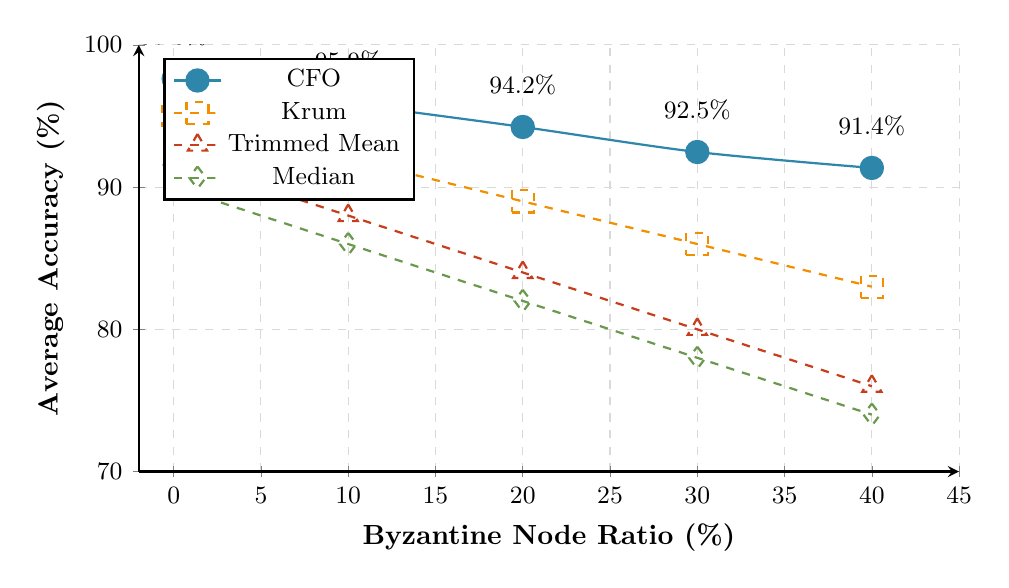
\begin{tikzpicture}
\begin{axis}[
    width=12cm,
    height=7cm,
    xlabel={Byzantine Node Ratio (\%)},
    ylabel={Average Accuracy (\%)},
    xmin=-2, xmax=45,
    ymin=70, ymax=100,
    grid=both,
    grid style={dashed, gray!30},
    axis lines=left,
    axis line style={thick},
    legend pos=north west,
    thick
]

% CFO method
\addplot[
    color=cfoBlue,
    mark=*,
    mark size=4pt,
    thick,
    smooth
] coordinates {
    (0,97.62)
    (10,95.88)
    (20,94.23)
    (30,92.47)
    (40,91.35)
};
\addlegendentry{CFO}

% Krum method
\addplot[
    color=krumOrange,
    mark=square,
    mark size=4pt,
    dashed,
    smooth
] coordinates {
    (0,95)
    (10,92)
    (20,89)
    (30,86)
    (40,83)
};
\addlegendentry{Krum}

% Trimmed Mean method
\addplot[
    color=trimmedRed,
    mark=triangle,
    mark size=4pt,
    dashed,
    smooth
] coordinates {
    (0,92)
    (10,88)
    (20,84)
    (30,80)
    (40,76)
};
\addlegendentry{Trimmed Mean}

% Median method
\addplot[
    color=medianGreen,
    mark=diamond,
    mark size=4pt,
    dashed,
    smooth
] coordinates {
    (0,90)
    (10,86)
    (20,82)
    (30,78)
    (40,74)
};
\addlegendentry{Median}

% 添加CFO数据点标签
\node at (axis cs:0,97.62) [above=8pt] {97.6\%};
\node at (axis cs:10,95.88) [above=8pt] {95.9\%};
\node at (axis cs:20,94.23) [above=8pt] {94.2\%};
\node at (axis cs:30,92.47) [above=8pt] {92.5\%};
\node at (axis cs:40,91.35) [above=8pt] {91.4\%};

\end{axis}
\end{tikzpicture}
\caption{Relationship between Byzantine Tolerance and Prediction Accuracy. CFO maintains high accuracy even beyond traditional 33.3\% BFT limit.}
\label{fig:tolerance_trend}
\end{figure}

\section{Technical Innovation Capability Radar Chart}

\begin{figure}[H]
\centering
\begin{tikzpicture}
\begin{polaraxis}[
    width=10cm,
    height=10cm,
    ymin=0, ymax=5,
    ytick={0,1,2,3,4,5},
    yticklabels={0,1,2,3,4,5},
    xtick={0,1.256637,2.513274,3.769911,5.026548},
    xticklabels={Spectral\\Analysis,Delta\\Response,High-Dim\\Clustering,Median\\Bootstrapping,LLM\\Integration},
    grid=both,
    major grid style={dashed, gray!50},
    minor tick num=4,
    minor grid style={dotted, gray!30},
    title={Technical Innovation Capability Radar Chart},
    title style={font=\bfseries\large},
    legend pos=outer north east
]

% CFO method
\addplot[
    color=cfoBlue,
    mark=*,
    mark size=4pt,
    thick,
    smooth
] coordinates {
    (0,5)
    (1.256637,5)
    (2.513274,5)
    (3.769911,5)
    (5.026548,5)
    (0,5)
};
\addlegendentry{CFO}

% Traditional BFT
\addplot[
    color=krumOrange,
    mark=square,
    mark size=4pt,
    dashed,
    smooth
] coordinates {
    (0,0)
    (1.256637,0)
    (2.513274,1)
    (3.769911,0)
    (5.026548,0)
    (0,0)
};
\addlegendentry{Traditional BFT}

% Federated Defense
\addplot[
    color=trimmedRed,
    mark=triangle,
    mark size=4pt,
    dashed,
    smooth
] coordinates {
    (0,1)
    (1.256637,0)
    (2.513274,2)
    (3.769911,2)
    (5.026548,0)
    (0,1)
};
\addlegendentry{Federated Defense}

\end{polaraxis}
\end{tikzpicture}
\caption{Technical Innovation Capability Radar Chart showing CFO's comprehensive capabilities across all technical dimensions.}
\label{fig:radar_chart}
\end{figure}

\section{Detailed Comparison Tables}

\begin{figure}[H]
\centering
\begin{subfigure}{0.95\textwidth}
\centering
\begin{tabular}{|c|c|c|c|c|c|}
\hline
\rowcolor{cfoBlue}
\textcolor{white}{\textbf{Method}} & \textcolor{white}{\textbf{Byzantine Tolerance}} & \textcolor{white}{\textbf{Avg Accuracy}} & \textcolor{white}{\textbf{Consensus Delay}} & \textcolor{white}{\textbf{Communication}} & \textcolor{white}{\textbf{Application}} \\
\hline
\rowcolor{E8F4F8}
\textbf{CFO} & \textbf{40\%} & \textbf{94.08\%} & \textbf{$\sim$3.5 s*} & \textbf{O(n²)} & \textbf{Multi-Agent Prediction} \\
\hline
PBFT & 33.3\% & - & 2-5 s & O(n²) & Blockchain/Database \\
\hline
HotStuff & 33.3\% & - & 1-3 s & O(n) & Blockchain \\
\hline
Tendermint & 33.3\% & - & 1-10 s & O(n²) & Blockchain \\
\hline
BFT-SMaRt & 33.3\% & - & 5-20 ms & O(n³) & Distributed Systems \\
\hline
\end{tabular}
\caption{Traditional BFT Consensus Methods}
\end{subfigure}

\vspace{1cm}

\begin{subfigure}{0.95\textwidth}
\centering
\begin{tabular}{|c|c|c|c|c|c|}
\hline
\rowcolor{cfoBlue}
\textcolor{white}{\textbf{Method}} & \textcolor{white}{\textbf{Byzantine Tolerance}} & \textcolor{white}{\textbf{Avg Accuracy}} & \textcolor{white}{\textbf{Consensus Delay}} & \textcolor{white}{\textbf{Communication}} & \textcolor{white}{\textbf{Application}} \\
\hline
\rowcolor{E8F4F8}
\textbf{CFO} & \textbf{40\%} & \textbf{94.08\%} & \textbf{$\sim$3.5 s*} & \textbf{O(n²)} & \textbf{Multi-Agent Prediction} \\
\hline
Krum & 50\% & 85\% & - & Low & Federated Learning \\
\hline
Trimmed Mean & 50\% & 80\% & - & Low & Federated Learning \\
\hline
Median & 50\% & 80\% & - & Low & Federated Learning \\
\hline
Multi-Krum & 50\% & 90\% & - & Medium & Federated Learning \\
\hline
Bulyan & 50\% & 88\% & - & High & Federated Learning \\
\hline
\end{tabular}
\caption{Federated Learning Byzantine Defense Methods}
\end{subfigure}
\caption{Detailed Comparison with Existing Methods. *CFO: $\sim$3.5s for consensus algorithm (excluding 60-90s for 30 sequential LLM API calls).}
\label{fig:comparison_tables}
\end{figure}

\end{document}